\documentclass[conference]{IEEEtran}
\usepackage[utf8]{inputenc}
\usepackage[T1]{fontenc}
\usepackage[spanish,es-tabla]{babel}
\usepackage{amsmath,amssymb}
\usepackage{graphicx}
\usepackage{booktabs}
\usepackage{array}
\usepackage{tabularx}
\usepackage{float}      % habilita [H]: la figura/tabla queda exactamente donde se escribe
\usepackage{siunitx}
\usepackage{xcolor}
\usepackage{hyperref}

\sisetup{output-decimal-marker={.}}
\graphicspath{{figuras/}{../../../MODELOS/PISTON/figuras/}}

% Columnas para tabularx: X = ajusta al ancho disponible y parte líneas
\newcolumntype{L}{>{\raggedright\arraybackslash}X}
\newcolumntype{C}{>{\centering\arraybackslash}X}
\renewcommand{\arraystretch}{1.15}

% Marcas de trabajo pendiente: se buscan con "PENDIENTE" antes de entregar
\newcommand{\pendiente}[1]{\textcolor{red}{[PENDIENTE: #1]}}
\newcommand{\figpendiente}[2]{%
  \fbox{\parbox[c][#1][c]{0.95\columnwidth}{\centering\textcolor{red}{[FIGURA PENDIENTE]}\\\small #2}}}

% REGLAS DE LA PLANTILLA (las mismas del informe de la validación unitaria)
% - Toda tabla usa tabularx con ancho \columnwidth.
% - Toda figura y tabla usa [H].
% - Las imágenes van con width=\columnwidth (o menos); figure* para las anchas.

\begin{document}

\title{MARLUP: Actividad 3 -- Processor-in-the-Loop\\de la plataforma completa}

\author{
\IEEEauthorblockN{Aarón Salas Alvarado, Mónica Solís Murillo, Eduardo Valle Arriola}
\IEEEauthorblockA{Instituto Tecnológico de Costa Rica\\
Laboratorio de Control Automático, Prof. Adolfo Chaves Jiménez}
}

\maketitle

% =====================================================================
% 150--200 palabras al final: qué se hizo, resultado principal con números,
% causa principal de la degradación.
\begin{abstract}
Se extendió la validación \textit{Processor-in-the-Loop} (PiL) de MARLUP, una plataforma de nivelación con tres cilindros hidráulicos, de un actuador a la planta completa. La plataforma, el oleaje de Pierson--Moskowitz ($H_s=\SI{2}{m}$, $T_p=\SI{10}{s}$) y los actuadores se simulan en Simulink, y los tres controladores PI de posición se ejecutan en un Arduino UNO con código generado por Embedded Coder. La función de transferencia del actuador se identificó sobre el modelo no lineal, y con ella se diseñó un único PI ($K_p=20$, $K_i=1$) que cumple las especificaciones de respuesta al escalón ($M_p=\SI{2.4}{\percent}$, $t_s=\SI{0.28}{s}$) con márgenes de \SI{16.9}{dB} y \SI{73.7}{\degree}. Con una ganancia de nivelación $K=15$, la inclinación pico de la mesa baja de \SI{2.88}{\degree} a \SI{0.78}{\degree} en \textit{pitch} y de \SI{1.52}{\degree} a \SI{0.42}{\degree} en \textit{roll}, por debajo del requisito de \SI{1}{\degree}. El PiL reproduce al \textit{Model-in-the-Loop} (MiL) con error nulo. Con cuatro no idealidades del encoder lineal, modeladas en la realimentación (linealidad, histéresis, ADC de 10 bits y ruido de 5 LSB), el comando de las válvulas adquiere un ruido de \num{0.058} RMS y la inclinación de la mesa uno de \SI{0.04}{\degree} RMS, y el pico de \textit{pitch} sube a \SI{0.82}{\degree}. Con oleajes más agresivos ($T_p$ más corto), el mismo controlador deja la mesa en \SI{1.46}{\degree} con una base de \SI{5}{\degree} y pierde la nivelación con \SIlist{10;15}{\degree}, porque el comando de ángulo y las válvulas se saturan. La causa es que la mesa realiza solo $g=R_T/R_B=0.188$ del ángulo ordenado, por una diferencia entre la cinemática inversa y las uniones del ensamble.
\end{abstract}

\begin{IEEEkeywords}
Processor-in-the-Loop, control hidráulico, plataforma de nivelación, oleaje, MARLUP.
\end{IEEEkeywords}

% =====================================================================
\section{Introducción}
% Del PiL unitario (un pistón) al PiL de la planta completa.
MARLUP es una plataforma que nivela su mesa (\textit{roll} y \textit{pitch}) frente al movimiento de una base excitada por el oleaje, mediante tres cilindros hidráulicos \cite{wang2025}. En una primera etapa se validó el controlador de posición de un solo actuador mediante un esquema \textit{Processor-in-the-Loop} (PiL), con resultados documentados en el informe de validación unitaria \cite{pil_unitario}. En la presentación se solicitó extender el PiL a la planta completa: los tres controladores de posición se ejecutan en un mismo microcontrolador mientras la plataforma, el oleaje y los actuadores se simulan en Simulink. Este informe documenta esa integración.

El objetivo es verificar que el controlador de los tres actuadores, ejecutado en el microcontrolador, mantiene la mesa nivelada frente a un oleaje que inclina la base varios grados. El requisito de desempeño es mantener la inclinación de la mesa por debajo de \SI{1}{\degree} en \textit{roll} y en \textit{pitch} con un oleaje de $H_s=\SI{2}{m}$.

La Sec.~\ref{sec:correcciones} responde a las observaciones de la presentación. La Sec.~\ref{sec:modelo} presenta el modelo de la planta, la función de transferencia del actuador y el diseño del controlador. Las Secs.~\ref{sec:interfaz}, \ref{sec:control} y \ref{sec:pil} describen la interfaz con el microcontrolador, la implementación del controlador y la arquitectura PiL. Las Secs.~\ref{sec:ideal} y \ref{sec:noideal} presentan las implementaciones con sensores ideales y no ideales, y la Sec.~\ref{sec:resultados} las compara.

% =====================================================================
\section{Correcciones de la presentación}
\label{sec:correcciones}
% Criterio R1: cada observación con su acción y su evidencia.
\begin{table}[H]
\centering
\caption{Observaciones de la presentación y acciones tomadas}
\label{tab:correcciones}
\small
\begin{tabularx}{\columnwidth}{LLL}
\toprule
Observación & Acción & Evidencia \\
\midrule
El PiL incluía un solo pistón & Se integraron los tres controladores en un solo MCU, con un único bloque Model en modo PIL y código generado por Embedded Coder & Secs.~\ref{sec:pil} y \ref{sec:ideal} \\
\pendiente{observación} & \pendiente{acción} & \pendiente{sección} \\
\bottomrule
\end{tabularx}
\end{table}

% =====================================================================
\section{Modelo matemático de la planta}
\label{sec:modelo}
% Criterio C1: consistente con la Actividad 2, parámetros, unidades y puntos de operación.

\subsection{Arquitectura del sistema}
La Fig.~\ref{fig:cascada} resume el sistema. El oleaje mueve la base en \textit{heave}, \textit{pitch} y \textit{roll} ($z_b$, $\theta_b$, $\alpha_b$). Un lazo exterior de nivelación calcula la orientación que debe tener la mesa respecto de la base; la cinemática inversa la convierte en la elongación de referencia de cada cilindro, y tres lazos PI de posición, uno por actuador, mueven los cilindros. La plataforma se modela en Simscape Multibody, que devuelve a cada actuador su fuerza de carga $F_{L,i}$.

\begin{figure*}[t]
\centering
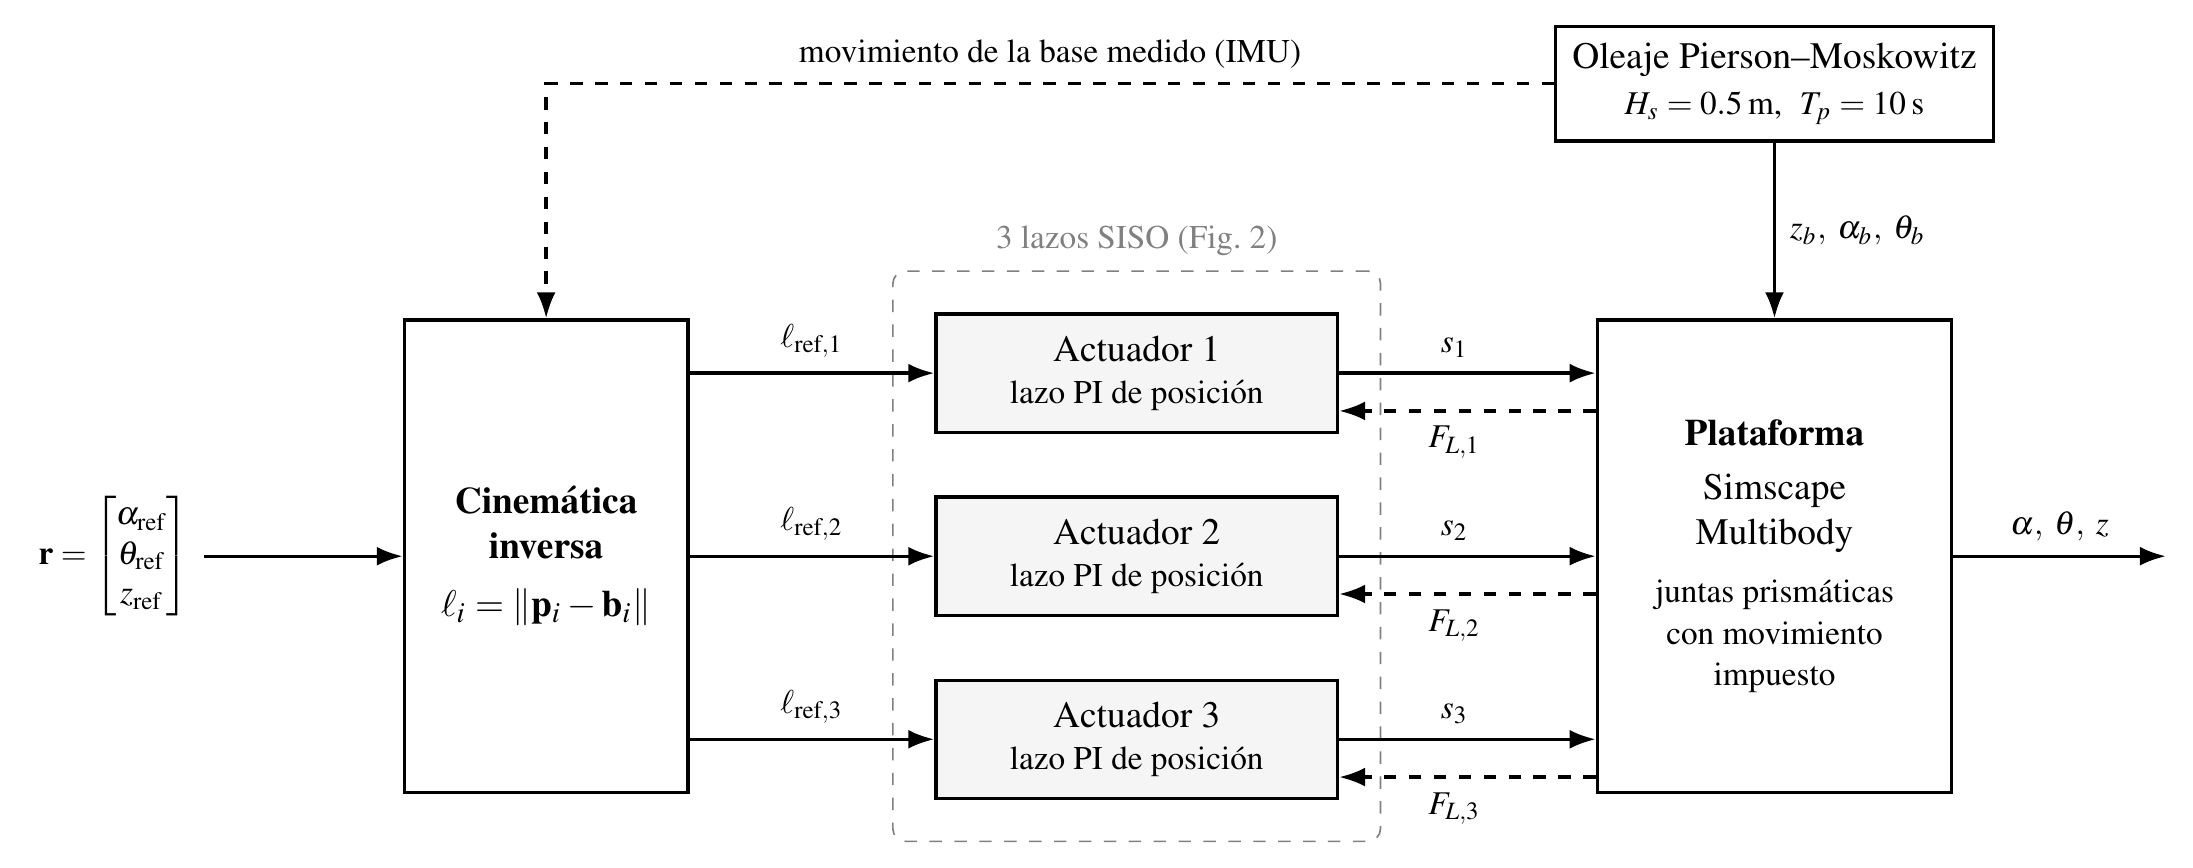
\includegraphics[width=0.85\textwidth]{fig3_cascada_marlup.png}
\caption{Estructura en cascada de MARLUP: cinemática inversa, tres lazos de posición y plataforma. \pendiente{actualizar: en el modelo actual el lazo exterior realimenta el ángulo medido de la mesa con una ganancia $K$ (Sec.~\ref{sec:ganancias}); no usa el movimiento de la base como prealimentación.}}
\label{fig:cascada}
\end{figure*}

En el modelo de Simulink (\texttt{Model\_aaronC.slx}), el lazo exterior es proporcional sobre el ángulo medido de la mesa:
\begin{equation}
\alpha_c = \operatorname{sat}_{\pm0.6}\!\big(K(\alpha_{ref}-\alpha)\big),\qquad
\theta_c = \operatorname{sat}_{\pm0.6}\!\big(K(\theta_{ref}-\theta)\big),
\label{eq:lazo_ext}
\end{equation}
con $K=15$, $\alpha_{ref}=\theta_{ref}=0$ y los comandos en radianes. El lazo de \textit{heave} está desactivado ($K_z=0$), de modo que la altura comandada es la nominal $z_c=Z_0$.

\subsection{Oleaje: espectro de Pierson--Moskowitz}
El estado de mar se describe con el espectro de Pierson--Moskowitz \cite{pierson1964} expresado con la altura significativa $H_s$ y el periodo pico $T_p$:
\begin{equation}
S(f)=\frac{5}{16}\,H_s^2\,f_p^4\,f^{-5}\exp\!\left[-\frac{5}{4}\left(\frac{f_p}{f}\right)^{4}\right],\qquad f_p=\frac{1}{T_p},
\label{eq:pm}
\end{equation}
con $H_s=\SI{2}{m}$ (estado de mar 4) y $T_p=\SI{10}{s}$. La superficie se sintetiza como una suma de $N=100$ frecuencias entre $\Delta f$ y $4f_p$ y $M=50$ direcciones, con fases aleatorias $\varphi_{nm}$ fijas (semilla 42, para que todas las corridas vean el mismo mar):
\begin{equation}
\eta(x,y,t)=\sum_{n=1}^{N}\sum_{m=1}^{M}A_{nm}\cos\!\big(\mathbf{k}_{nm}\!\cdot\mathbf{r}-\omega_n t+\varphi_{nm}\big),
\label{eq:eta}
\end{equation}
\begin{equation}
A_{nm}=\sqrt{2\,S(f_n)\,D(\beta_m)\,\Delta f\,\Delta\beta},\qquad k_n=\frac{\omega_n^2}{g},
\end{equation}
donde $\mathbf{r}=(x,y)$, $\mathbf{k}_{nm}=k_n(\cos\beta_m,\sin\beta_m)$, $k_n$ sale de la relación de dispersión en aguas profundas y $D(\beta)=\frac{2}{\pi}\cos^{2s}(\beta/2)$, con $s=10$, es la dispersión direccional. El movimiento de la base se toma en el origen: el \textit{heave} es $z_b=\eta(0,0,t)$ y los ángulos son las pendientes de la superficie,
\begin{equation}
\theta_b=-\arctan\frac{\partial\eta}{\partial x}\Big|_{0},\qquad \alpha_b=-\arctan\frac{\partial\eta}{\partial y}\Big|_{0}.
\label{eq:pendientes}
\end{equation}
Es decir, la base de la plataforma se apoya en el plano tangente a la superficie del mar en el origen: su eje $z_b$ es la normal a $\eta$ en ese punto, y la perturbación que ve el lazo de nivelación son las derivadas parciales de la superficie, evaluadas allí en cada instante. La Fig.~\ref{fig:espectro} muestra el espectro, su discretización, una realización de la superficie y ese plano tangente con el marco de la base.

\begin{figure*}[t]
\centering
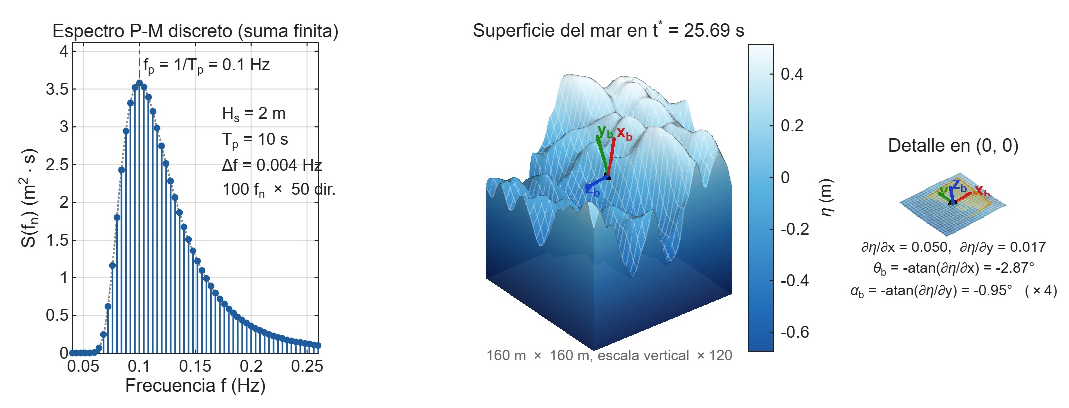
\includegraphics[width=0.9\textwidth]{espectro_pm.pdf}
\caption{Oleaje de Pierson--Moskowitz con $H_s=\SI{2}{m}$ y $T_p=\SI{10}{s}$. Izquierda: espectro discreto del modelo, una línea $S(f_n)$ por cada una de las 100 frecuencias de la suma finita~\eqref{eq:eta} (puntos); la curva punteada es el espectro continuo~\eqref{eq:pm} como referencia. Centro: superficie $\eta(x,y,t^*)$ de la misma realización que ve la simulación, en el instante $t^*$ del pico de \textit{pitch} de la base, con el marco de la base $(x_b,y_b,z_b)$ en el punto de medición; escala vertical exagerada. Derecha: detalle del plano tangente en $(0,0)$: sus pendientes $\partial\eta/\partial x$ y $\partial\eta/\partial y$ son la perturbación~\eqref{eq:pendientes} que recibe la plataforma. Generada con \texttt{figuras/fig\_espectro\_pm.m}.}
\label{fig:espectro}
\end{figure*}

\pendiente{Revisar la dispersión direccional del bloque \texttt{P-M SPECTRUM}: como $\beta\in(0,2\pi]$, el recorte \texttt{theta > pi/2} deja activas solo las direcciones entre \SI{0}{\degree} y \SI{90}{\degree}, y $\int D\,d\beta\approx0.31$ en lugar de 1. La superficie simulada tiene $4\sigma_\eta=4\sqrt{\sum A_{nm}^2/2}\approx\SI{1.12}{m}$ en lugar de $H_s=\SI{2}{m}$; por eso se usa $H_s=\SI{2}{m}$, para tener una perturbación considerable.}

Con este estado de mar y el lazo de nivelación apagado ($K=0$), la mesa sigue a la base y se inclina hasta \SI{2.88}{\degree} en \textit{pitch} (\SI{1.43}{\degree} RMS) y hasta \SI{1.52}{\degree} en \textit{roll} (\SI{0.56}{\degree} RMS), casi el triple del requisito.

\subsection{Cinemática inversa}
La mesa (marco $P$) se ubica respecto de la base con
\begin{equation}
T_0^P=\operatorname{Trasl}(0,0,z)\,R_y(\theta)\,R_x(\alpha),
\end{equation}
y la longitud del cilindro $i$ es la distancia entre sus rótulas:
\begin{equation}
\ell_i=\big\lVert R_y(\theta)R_x(\alpha)\,\mathbf{p}_i+z\,\hat{\mathbf{k}}-\mathbf{b}_i\big\rVert,\qquad i=1,2,3,
\label{eq:ik}
\end{equation}
con $\mathbf{b}_i=R_B(\cos\phi_i,\sin\phi_i,0)$ y $\mathbf{p}_i=R_T(\cos\phi_i,\sin\phi_i,0)$, $\phi_i\in\{\SI{-30}{\degree},\SI{90}{\degree},\SI{210}{\degree}\}$. Cada pata es una cadena rótula--cilindro--rótula en la que las rótulas solo aportan orientación, de modo que la longitud del cilindro es exactamente la norma del vector $\mathbf{d}_i=\mathbf{p}_i-\mathbf{b}_i$ entre ambos anclajes (Fig.~\ref{fig:cinematica}). La geometría se midió en el ensamblaje CAD (Tabla~\ref{tab:geometria}).

\begin{figure*}[t]
\centering
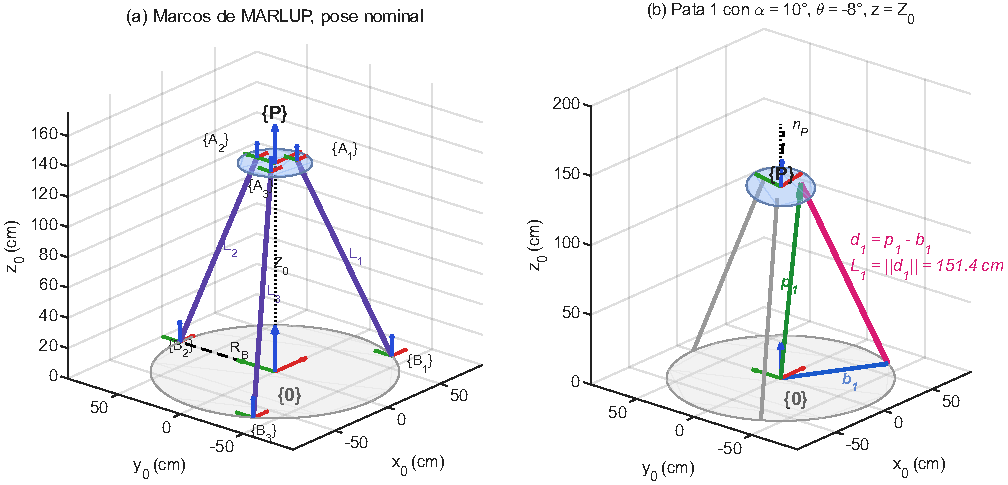
\includegraphics[width=0.9\textwidth]{cinematica.pdf}
\caption{Modelo cinemático de MARLUP. (a) Marco de la base $\{0\}$, de la mesa $\{P\}$ y de los anclajes inferiores $\{B_i\}$ y superiores $\{A_i\}$, en la pose nominal; los cilindros definen las longitudes $L_1$, $L_2$ y $L_3$. (b) Construcción vectorial de~\eqref{eq:ik} sobre la pata 1: $\mathbf{b}_1$ ubica el anclaje inferior (fijo), $\mathbf{p}_1$ el superior (móvil con la pose) y $L_1$ es la norma de su diferencia; $\mathbf{n}_P$ es la normal de la mesa. Ejes $x$, $y$, $z$ de cada marco en rojo, verde y azul. Generada con \texttt{figuras/fig\_cinematica.m}.}
\label{fig:cinematica}
\end{figure*} La referencia de cada lazo de posición es
\begin{equation}
x_{ref,i}=\ell_i-\ell_0+x_0,\qquad \ell_0=\sqrt{(R_B-R_T)^2+Z_0^2},
\end{equation}
donde $x_0=\SI{0.23}{m}$ ubica cada vástago cerca de la mitad de su carrera de \SI{0.45}{m}, de modo que puede extenderse o retraerse.

\begin{table}[H]
\centering
\caption{Geometría de los anclajes}
\label{tab:geometria}
\small
\begin{tabularx}{\columnwidth}{lLr}
\toprule
Símbolo & Descripción & Valor \\
\midrule
$R_B$ & Radio de los anclajes inferiores & \SI{0.7608}{m} \\
$R_T$ & Radio de los anclajes superiores & \SI{0.143}{m} \\
$Z_0$ & Separación vertical nominal & \SI{1.377}{m} \\
$\ell_0$ & Longitud nominal entre rótulas & \SI{1.509}{m} \\
$x_0$ & Posición de trabajo del vástago & \SI{0.23}{m} \\
\bottomrule
\end{tabularx}
\end{table}

Linealizando \eqref{eq:ik} en la pose nominal se obtiene el jacobiano que relaciona ángulos de la mesa con elongaciones:
\begin{equation}
\Delta\boldsymbol{\ell}\approx
\underbrace{\begin{bmatrix}-0.065 & -0.113 & 0.912\\ 0.130 & 0 & 0.912\\ -0.065 & 0.113 & 0.912\end{bmatrix}}_{J}
\begin{bmatrix}\Delta\alpha\\ \Delta\theta\\ \Delta z\end{bmatrix},
\label{eq:jacobiano}
\end{equation}
con $\Delta\alpha$, $\Delta\theta$ en radianes y $\Delta\boldsymbol{\ell}$, $\Delta z$ en metros. Un grado de inclinación exige apenas unos \SI{2}{mm} de elongación, lo que fija la resolución de posición que necesita el sistema (Sec.~\ref{sec:ganancias}).

\subsection{Actuador electrohidráulico}
Cada actuador es un cilindro de doble efecto Bosch Rexroth CDH1 de \SI{40}{mm} de pistón y \SI{28}{mm} de vástago \cite{rexroth}, comandado por una válvula proporcional 4/3 (Fig.~\ref{fig:hidraulico}). El modelo es el mismo de la validación unitaria \cite{pil_unitario} y se resume en la Fig.~\ref{fig:bloques}.

\begin{figure}[H]
\centering
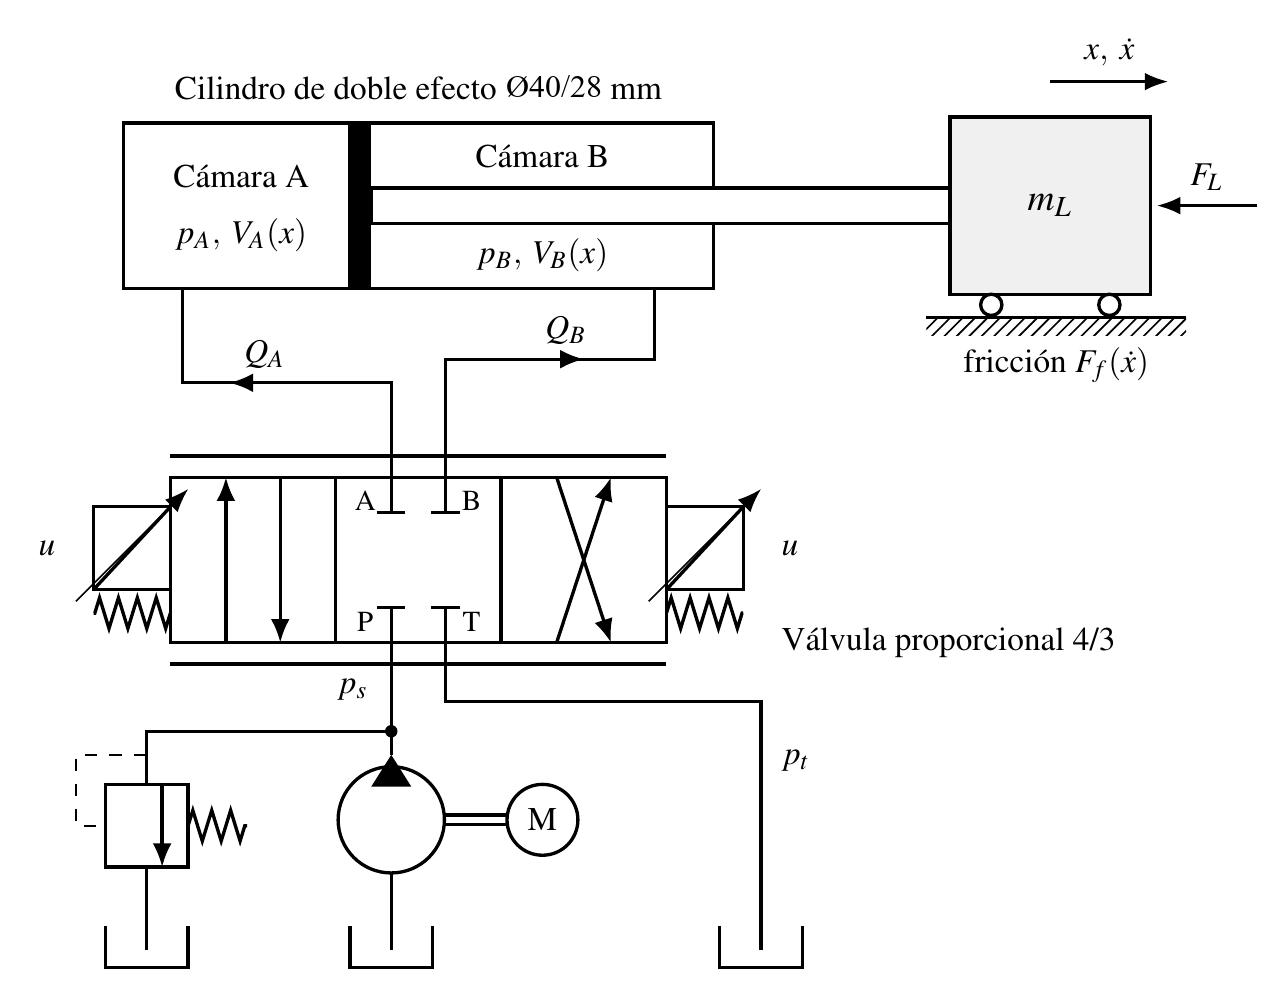
\includegraphics[width=0.85\columnwidth]{fig1_esquema_hidraulico.png}
\caption{Esquema hidráulico de un actuador. \pendiente{corregir la etiqueta: el cilindro es Ø40/28, no Ø63/36.}}
\label{fig:hidraulico}
\end{figure}

\begin{figure*}[t]
\centering
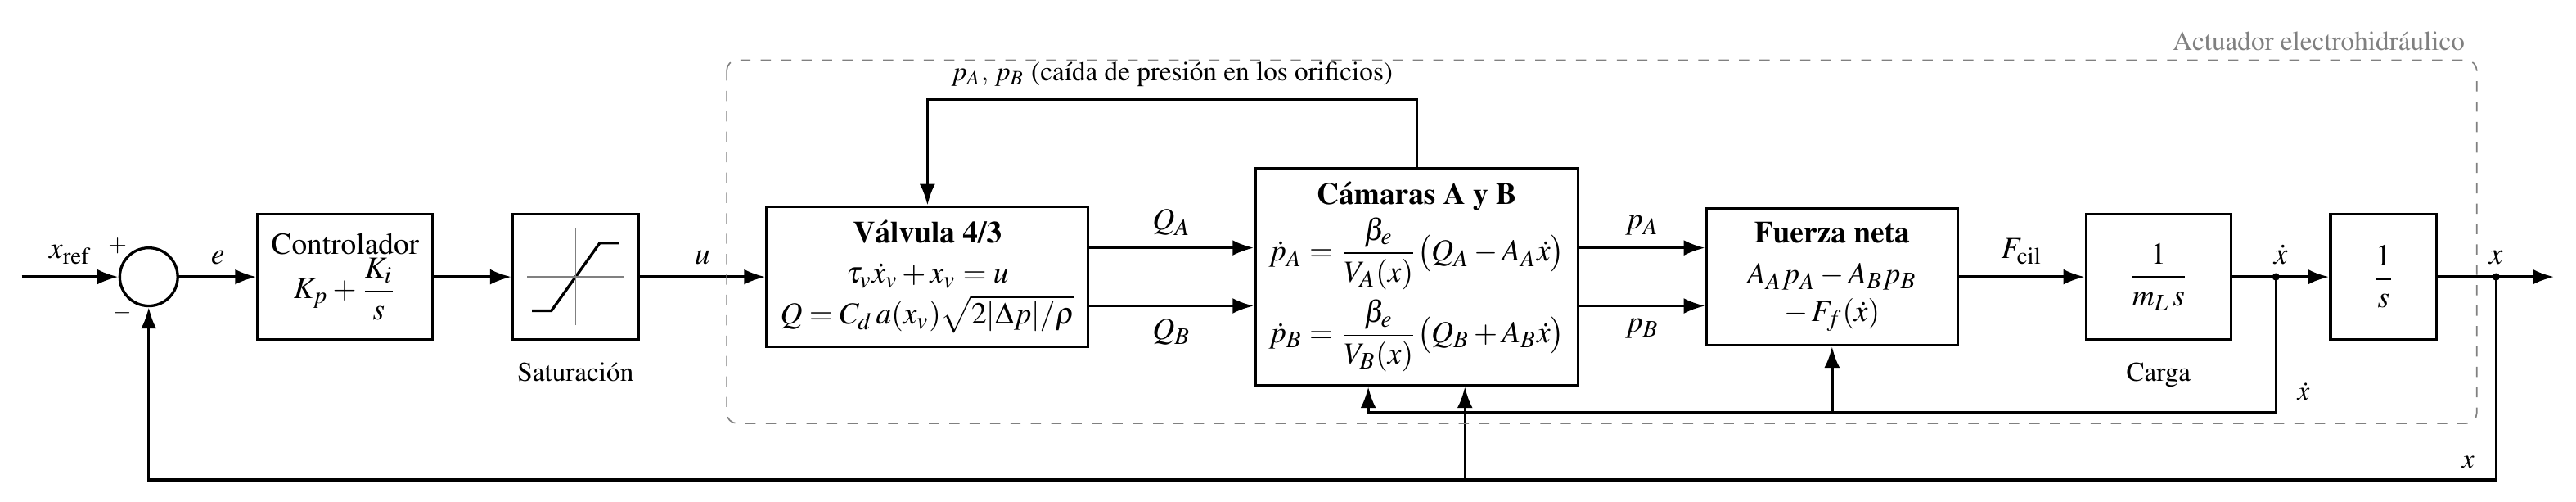
\includegraphics[width=\textwidth]{fig2_bloques_actuador.png}
\caption{Diagrama de bloques del lazo de posición de un actuador.}
\label{fig:bloques}
\end{figure*}

\textit{Válvula.} Se modela como un sistema de primer orden con retardo, y el caudal por cada orificio sigue la ecuación de orificio:
\begin{equation}
\tau_v\dot x_v+x_v=u,\qquad Q=C_d\,a(x_v)\sqrt{2|\Delta p|/\rho}\,\operatorname{sgn}(\Delta p).
\end{equation}

\textit{Cámaras.} La continuidad con compresibilidad del aceite da
\begin{equation}
\dot p_A=\frac{\beta_e}{V_A(x)}\big(Q_A-A_A\dot x\big),\qquad
\dot p_B=\frac{\beta_e}{V_B(x)}\big(Q_B+A_B\dot x\big).
\end{equation}

\textit{Carga.} El balance de fuerzas sobre la masa móvil es
\begin{equation}
m_L\ddot x=A_Ap_A-A_Bp_B-F_f(\dot x)-F_L,
\end{equation}
donde $F_L$ es la fuerza que impone la plataforma (Simscape Multibody). La Tabla~\ref{tab:hidraulica} reúne los parámetros, tomados de \texttt{MARLUP\_hydr\_params.m}.

\begin{table}[H]
\centering
\caption{Parámetros del actuador}
\label{tab:hidraulica}
\small
\begin{tabularx}{\columnwidth}{lLr}
\toprule
Símbolo & Descripción & Valor \\
\midrule
$m_L$ & Masa móvil por actuador & \SI{20}{kg} \\
$b$ & Fricción viscosa & \SI{1000}{N.s/m} \\
$\beta_e$ & Módulo de compresibilidad efectivo & \SI{750}{MPa} \\
$A_A$, $A_B$ & Áreas del lado del pistón y del vástago & \SI{12.57}{cm^2}, \SI{6.41}{cm^2} \\
$V_{A0}$, $V_{B0}$ & Volúmenes muertos & \SI{0.30}{L}, \SI{0.15}{L} \\
$p_s$ & Presión de suministro & \SI{160}{bar} \\
$Q_N$ & Caudal nominal de la válvula (a \SI{35}{bar}) & \SI{40}{L/min} \\
$\tau_v$ & Constante de tiempo de la válvula (más \SI{1}{ms} de retardo) & \SI{2}{ms} \\
\bottomrule
\end{tabularx}
\end{table}

\textit{Función de transferencia.} Alrededor de $\dot x_0=0$, con volúmenes $V_{A0}$, $V_{B0}$, fricción viscosa $F_f\approx b\dot x$ y los coeficientes de la válvula $K_q=\partial Q/\partial x_v$ y $K_c=-\partial Q/\partial p$, la función de transferencia de comando a posición es
\begin{equation}
G(s)=\frac{X(s)}{U(s)}=\frac{K_q\big[(A_AC_B+A_BC_A)s+K_c(A_A+A_B)\big]}{s\,(\tau_vs+1)\,\Delta(s)},
\label{eq:G}
\end{equation}
\begin{multline}
\Delta(s)=(m_Ls+b)(C_As+K_c)(C_Bs+K_c)\\+A_A^2(C_Bs+K_c)+A_B^2(C_As+K_c),
\end{multline}
con $C_{A,B}=V_{A0,B0}/\beta_e$. La planta tiene un integrador: un comando constante produce una velocidad constante del vástago.

Los parámetros de~\eqref{eq:G} se obtuvieron con un ensayo en lazo abierto sobre el modelo no lineal de Simulink, en el punto de trabajo de la plataforma ($x_0=\SI{0.23}{m}$): escalones de $u=\pm0.02$, $\pm0.05$ y $\pm0.1$ en la válvula y medición de la velocidad del vástago. La velocidad se establece en unos \SI{25}{ms} sin oscilar, de modo que la dinámica hidráulica queda bien representada por un retardo y una constante de tiempo, y~\eqref{eq:G} se reduce a
\begin{equation}
G(s)\approx\frac{K_v\,e^{-\theta s}}{s\,(\tau s+1)}=\frac{0.636\,e^{-0.0088s}}{s\,(0.0085s+1)},
\label{eq:Gid}
\end{equation}
con los valores de la Tabla~\ref{tab:lineal}. El diseño usa~\eqref{eq:Gid} discretizada con retenedor de orden cero a $T_s=\SI{10}{ms}$, como la ve el controlador.

\begin{table}[H]
\centering
\caption{Parámetros de la función de transferencia identificada}
\label{tab:lineal}
\small
\begin{tabularx}{\columnwidth}{lLr}
\toprule
Símbolo & Significado & Valor \\
\midrule
$K_v$ & Velocidad por unidad de comando (señal pequeña) & \SI{0.636}{m/s} \\
 & \quad extensión / retracción & \num{0.740} / \SI{0.532}{m/s} \\
 & \quad a válvula abierta ($|u|=1$) & \num{0.43} / \SI{0.29}{m/s} \\
$\tau$ & Constante de tiempo de la velocidad & \SI{8.5}{ms} \\
$\theta$ & Retardo (válvula y compresibilidad) & \SI{8.8}{ms} \\
\bottomrule
\end{tabularx}
\end{table}

La asimetría entre extensión y retracción se debe a las áreas distintas del cilindro, y la caída de $K_v$ a válvula abierta, a la ecuación de orificio. $K_v$ es el promedio de los dos sentidos en señal pequeña, que es como trabaja el lazo durante la nivelación.

% ---------------------------------------------------------------------
\subsection{Diseño del controlador}
\label{sec:ganancias}

El sistema es una cascada: tres lazos internos de posición, uno por cilindro, y un lazo exterior de nivelación que cierra sobre el ángulo medido de la mesa.

\subsubsection{Lazo interno: posición de cada cilindro}

Se usa un PI $C(s)=K_p+K_i/s$ con integrador trapezoidal, anti-windup por \textit{clamping} y saturación del comando en $\pm1$. Las especificaciones son las del anteproyecto: sobrepaso $M_p\le\SI{10}{\percent}$, tiempo de establecimiento $t_s\le\SI{2}{s}$ (criterio del \SI{2}{\percent}) y error en régimen menor a \SI{2.3}{mm}, más márgenes de ganancia de al menos \SI{10}{dB} y de fase de al menos \SI{60}{\degree}. Las ganancias elegidas son
\begin{equation}
K_p=20\ \si{m^{-1}},\qquad K_i=1\ \si{m^{-1}.s^{-1}}.
\label{eq:pi}
\end{equation}
Con~\eqref{eq:Gid}, el lazo cruza en \SI{12.6}{rad/s}, con margen de fase de \SI{73.7}{\degree} y de ganancia de \SI{16.9}{dB}. El cruce es unas veinte veces la frecuencia pico del oleaje ($2\pi/T_p=\SI{0.63}{rad/s}$), donde el error de seguimiento del lazo cerrado es de \SI{4.9}{\percent}. El cero del PI ($K_i/K_p=\SI{0.05}{rad/s}$) queda dos décadas por debajo del cruce, así que la acción integral no reduce el margen de fase; su función es anular el error ante perturbaciones lentas, como la fuerza de carga o el sesgo de la válvula. La planta ya tiene un integrador, por lo que el lazo abierto es de tipo 2 y el error ante referencias constantes y rampas es nulo.

La Tabla~\ref{tab:temporal} y la Fig.~\ref{fig:escalon} muestran la respuesta al escalón con el modelo lineal y con el modelo no lineal completo, en dos condiciones: un escalón pequeño de \SI{10}{mm} en el punto de trabajo, representativo de la nivelación, y el escalón de 0 a \SI{0.40}{m} de la validación unitaria~\cite{pil_unitario}, en que la válvula satura. Las ganancias se eligieron con estas métricas, como el controlador de menor $t_s$ en el escalón pequeño que cumple todas las especificaciones en las tres respuestas; la comparación con los demás candidatos está en el repositorio (\texttt{MODELOS/PISTON/diseno\_pi.m}).

\begin{table}[H]
\centering
\caption{Respuesta al escalón del lazo interno con $K_p=20$, $K_i=1$}
\label{tab:temporal}
\footnotesize
\setlength{\tabcolsep}{3pt}
\begin{tabularx}{\columnwidth}{lCCCC}
\toprule
Respuesta & $M_p$ (\si{\percent}) & $t_r$ (\si{s}) & $t_s$ (\si{s}) & $|e_{ss}|$ (\si{mm}) \\
\midrule
Lineal~\eqref{eq:Gid} & 0.4 & 0.11 & 0.22 & 0 \\
No lineal, \SI{10}{mm} & 2.4 & 0.07 & 0.28 & 0.08 \\
No lineal, \SI{0.40}{m} & 0.1 & 0.73 & 0.96 & 0.19 \\
Requisito & $\le10$ & --- & $\le2$ & $<2.3$ \\
\bottomrule
\end{tabularx}
\end{table}

\begin{figure*}[t]
\centering
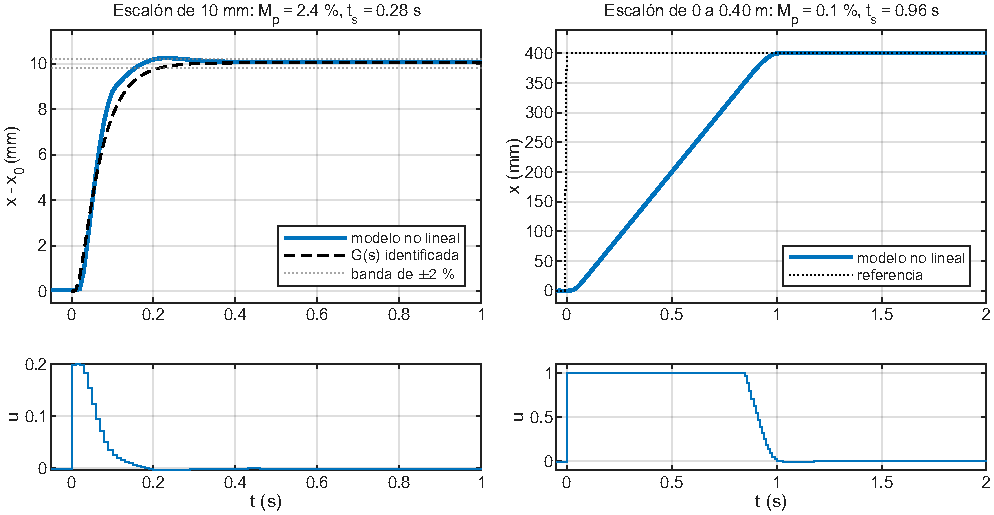
\includegraphics[width=0.85\textwidth]{pi_final_escalon.pdf}
\caption{Respuesta al escalón del lazo interno con $K_p=20$, $K_i=1$. Izquierda: escalón de \SI{10}{mm} en $x_0=\SI{0.23}{m}$, modelo no lineal y función de transferencia~\eqref{eq:Gid}. Derecha: escalón de 0 a \SI{0.40}{m}, en que la válvula satura y el pistón avanza a velocidad máxima. Abajo: comando de la válvula. Generada con \texttt{MODELOS/PISTON/figuras\_diseno\_pi.m}.}
\label{fig:escalon}
\end{figure*}

En el escalón grande la válvula satura y el tiempo lo fija el caudal máximo y no $K_p$: el pistón avanza a $\approx\SI{0.43}{m/s}$ y llega en \SI{0.96}{s}. El mismo controlador, ejecutado en el Arduino en la validación unitaria, da $M_p=\SI{0.13}{\percent}$, $t_s=\SI{0.96}{s}$ y $e_{ss}=\SI{0.20}{mm}$, idénticos al MiL.

\subsubsection{Lazo exterior: nivelación de la mesa}

\textit{Planta equivalente.} A la frecuencia del oleaje el lazo interno sigue su referencia, de modo que la cadena \emph{comando de ángulo $\rightarrow$ cinemática inversa $\rightarrow$ pistones $\rightarrow$ inclinación de la mesa} se comporta como una ganancia estática $g$, y la inclinación residual de la mesa es
\begin{equation}
\frac{\alpha(s)}{\alpha_b(s)}\approx\frac{1}{1+K\,g}.
\label{eq:sensibilidad}
\end{equation}
Idealmente $g=1$, pero la planta realiza una fracción del ángulo ordenado. El ajuste del barrido de $K$ (Fig.~\ref{fig:barrido}) da $g=0.184$, que reproduce las corridas con un error menor a \SI{0.2}{dB}. La causa es una diferencia entre la cinemática inversa y el ensamble de Simscape. La cinemática inversa supone que la mesa gira sobre su propio centro, con rótulas ideales arriba. En el ensamble, la unión superior de cada pata es un único pasador tangencial (el segundo eje de la cruceta está fijo), de modo que el eje de cada vástago queda en el plano radial de su anclaje inferior y la mesa gira alrededor del centro de la base. El brazo efectivo es entonces $R_B$ y no $R_T$, y $g=R_T/R_B=0.143/0.7608=0.188$, igual en \textit{roll} y en \textit{pitch}. Ese valor reproduce, sin ajuste, la atenuación medida para cada $K$ y el \SI{18}{\percent} del ángulo pedido que ya se había observado en la validación de la cinemática inversa \cite{avance2}. \pendiente{Decidir si se corrige la cinemática inversa ($g\approx1$), lo que obliga a reescalar $K$ y la saturación.} Por ese factor, el comando de ángulo debe ser unas cinco veces la inclinación que se quiere corregir, y su saturación se fijó en $\pm\SI{0.6}{rad}$. Con el límite anterior de $\pm\SI{0.1}{rad}$ el lazo solo podía compensar $0.1\,g\approx\SI{1}{\degree}$, y con el oleaje de $H_s=\SI{2}{m}$ la mesa quedaba por encima de \SI{2}{\degree} con cualquier $K$. El comando de \SI{0.6}{rad} pide unos \SI{80}{mm} de elongación, dentro de los $\pm\SI{220}{mm}$ de carrera libre alrededor de $x_0$.

\textit{Criterio de diseño.} Imponiendo que el pico de inclinación de la mesa quede bajo el requisito,
\begin{equation}
\frac{\theta_{base}}{1+Kg}\le\theta_{req}
\;\Longrightarrow\;
K\ge\frac{1}{g}\left(\frac{\theta_{base}}{\theta_{req}}-1\right).
\label{eq:Kmin}
\end{equation}
Con el pico sin compensar $\theta_{base}=\SI{2.88}{\degree}$, $\theta_{req}=\SI{1}{\degree}$ y $g=0.184$, resulta $K\ge10.2$.

\textit{Valor elegido.} $K=15$, que deja el pico de \textit{pitch} en \SI{0.78}{\degree}, un \SI{22}{\percent} por debajo del requisito. Subir a $K=20$ lo baja solo a \SI{0.64}{\degree}, a cambio de un \SI{9}{\percent} más de esfuerzo en las válvulas y de acercarse al límite de estabilidad: con este mismo PI, en el barrido previo con $H_s=\SI{0.5}{m}$, $K=30$ fue inestable.

\begin{figure*}[t]
\centering
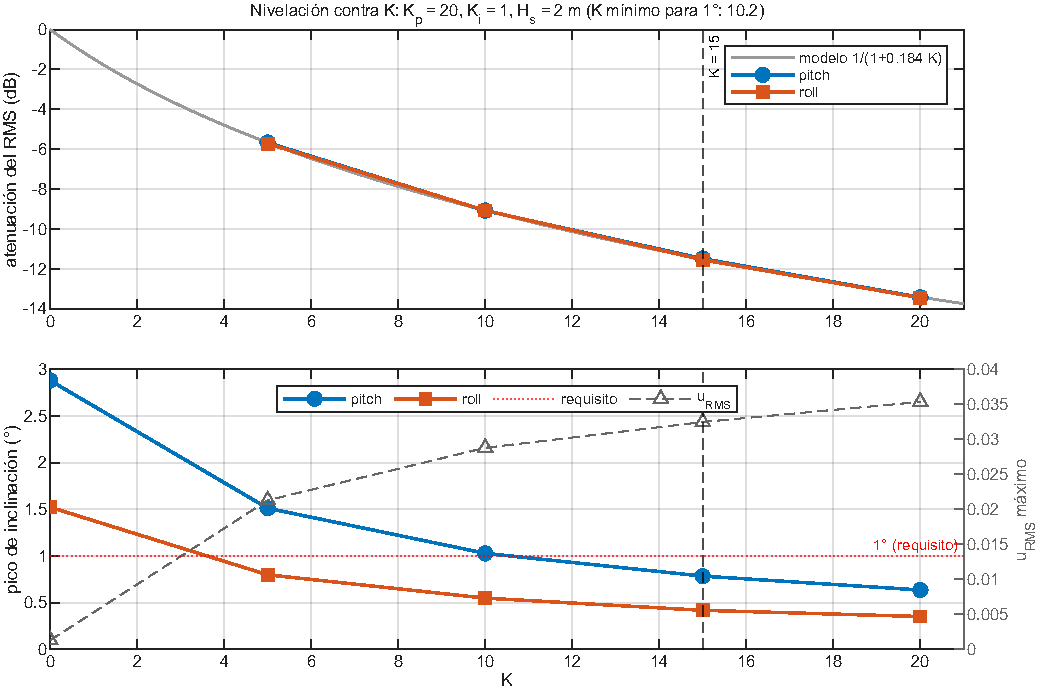
\includegraphics[width=0.8\textwidth]{barrido_k.pdf}
\caption{Nivelación contra la ganancia $K$ (MiL, $H_s=\SI{2}{m}$, sensor ideal). Arriba: atenuación del RMS de la inclinación y el modelo~\eqref{eq:sensibilidad} con $g=0.184$. Abajo: pico de inclinación frente al requisito de \SI{1}{\degree} y esfuerzo de control. Generada con \texttt{figuras/fig\_final.m}.}
\label{fig:barrido}
\end{figure*}

% =====================================================================
\section{Interfaz sensor/actuador -- MCU}
\label{sec:interfaz}
% Criterio C2: rangos de voltaje, resolución del ADC, PWM, escalamiento físico <-> cuentas.
Cada cilindro usa la misma cadena de conversión validada en el PiL unitario \cite{pil_unitario}: sensor magnetostrictivo de \SIrange{0}{10}{V} sobre \SI{450}{mm}, divisor 1:2, ADC de 10 bits (\SI{0.44}{mm} por cuenta) y comando de válvula de $\pm\SI{10}{V}$ generado con PWM de 8 bits ($\Delta u=2/256\approx0.0078$) y un amplificador.

En el modelo de Simulink, el transductor y la interfaz son dos subsistemas separados. El bloque \texttt{Linear encoder} está en el lazo de realimentación, entre cada cilindro y el controlador, y actúa solo sobre la posición medida: para cada uno de los tres cilindros, la posición pasa por un sesgo (error de linealidad), una histéresis (\textit{backlash}), un ruido aditivo independiente en cada cilindro, un cuantizador de \SI{0.44}{mm} (ADC) y una saturación al rango del ADC (\SIrange{0}{449.6}{mm}). La referencia no pasa por él. El subsistema \texttt{Interfaz MCU} muestrea la referencia y la posición medida a $T_s=\SI{10}{ms}$ y las convierte a precisión simple, que es el tipo que maneja el AVR; el error $e_i=x_{ref,i}-x_{m,i}$ se calcula dentro del controlador. El subsistema \texttt{Interfaz actuador} convierte el comando de vuelta a doble precisión y lo reparte a cada válvula. Con las no idealidades desactivadas, esos bloques son transparentes. Las unidades de la interfaz son metros para posición y referencia, y valor normalizado $u\in[-1,1]$ para el comando.

% =====================================================================
\section{Implementación del controlador en hardware}
\label{sec:control}
% Criterio C3: discretización, periodo justificado, código validado desde MATLAB, tiempo de ejecución.
Los tres PI se discretizan por Tustin con $T_s=\SI{10}{ms}$ y se implementan en forma posicional con anti-windup por \textit{clamping}, igual que en la validación unitaria:
\begin{equation}
\begin{aligned}
I_i[k] &= I_i[k-1]+\tfrac{K_iT_s}{2}\big(e_i[k]+e_i[k-1]\big),\\
u_i[k] &= \operatorname{sat}\big(K_p\,e_i[k]+I_i[k]\big),\qquad i=1,2,3.
\end{aligned}
\end{equation}
El periodo es muy menor que el tiempo de establecimiento del lazo interno (\SI{0.28}{s}) y que el periodo pico del oleaje (\SI{10}{s}). Los tres PI forman un solo modelo, \texttt{ctrl\_pi3.slx}, con las referencias y las posiciones como vectores de tres elementos en precisión simple; usan el bloque Discrete PID Controller de Simulink, como en la validación unitaria. Embedded Coder genera el código C a partir de ese modelo y lo compila para el ATmega328P, sin escribir firmware a mano. El mismo modelo se simula en el PC (MiL) con el bloque en modo normal y se ejecuta en la placa (PiL) con el bloque en modo PIL.

\pendiente{Tiempo de ejecución medido de los tres PI en el ATmega328P frente a los \SI{10}{ms} del periodo.}

% =====================================================================
\section{Arquitectura PiL y comunicación}
\label{sec:pil}
% Criterio C4: protocolo documentado, sincronización y latencia acotada.
La plataforma completa se simula en Simulink (\texttt{Model\_aaronC.slx}) y los tres PI se ejecutan en un Arduino UNO R3 mediante un único bloque Model en modo \textit{Processor-in-the-Loop} que referencia a \texttt{ctrl\_pi3} (Fig.~\ref{fig:bloquepil}). En cada periodo $T_s$, Simulink envía por el puerto serie las tres referencias y las tres posiciones medidas, el MCU ejecuta un paso del código generado y devuelve los tres comandos (Tabla~\ref{tab:interfazpil}). La simulación avanza solo cuando recibe la respuesta (\textit{lockstep}), por lo que la comunicación no se traslada a la planta. El enlace es de \SI{115200}{baud}; el programa lo carga y lo comunica el \textit{Simulink Support Package for Arduino Hardware}. En el AVR un \texttt{double} ocupa 4 bytes, por lo que la interfaz del controlador es de precisión simple.

\begin{table}[H]
\centering
\caption{Señales entre Simulink y el MCU en cada periodo}
\label{tab:interfazpil}
\small
\begin{tabularx}{\columnwidth}{llLr}
\toprule
Sentido & Señal & Contenido & Datos \\
\midrule
Simulink $\rightarrow$ MCU & \texttt{ref} & Referencia de los tres cilindros [m] & $3\times4$ B \\
Simulink $\rightarrow$ MCU & \texttt{x} & Posición medida (tras el ADC) [m] & $3\times4$ B \\
MCU $\rightarrow$ Simulink & \texttt{u} & Comando de las tres válvulas, en $[-1,1]$ & $3\times4$ B \\
\bottomrule
\end{tabularx}
\end{table}

Por cada periodo viajan 36 bytes de carga útil, es decir, al menos $36\cdot10/115200\approx\SI{3.1}{ms}$ de los \SI{10}{ms} del periodo, sin contar el encabezado del protocolo de Simulink. \pendiente{Latencia medida de un paso PiL.}

\begin{figure}[H]
\centering
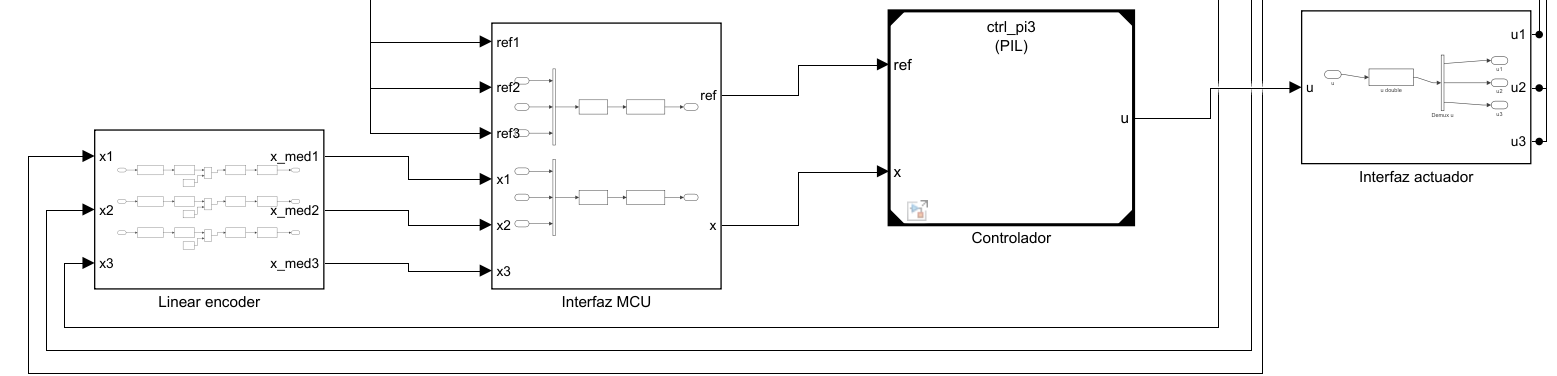
\includegraphics[width=\columnwidth]{pil_bloques.png}
\caption{Arquitectura PiL de la plataforma completa (nivel principal de \texttt{Model\_aaronC.slx}): las posiciones de los tres cilindros vuelven por el \texttt{Linear encoder}, la \texttt{Interfaz MCU} las muestrea junto con las referencias, el bloque \texttt{Controlador} ejecuta \texttt{ctrl\_pi3} en el Arduino y la \texttt{Interfaz actuador} reparte el comando a las válvulas.}
\label{fig:bloquepil}
\end{figure}

% =====================================================================
\section{Implementación 1: sensores y actuadores ideales}
\label{sec:ideal}
% Criterio C5: PiL ideal frente al MiL con una métrica definida.
Con sensores y actuadores ideales se simularon \SI{30}{s} de oleaje ($H_s=\SI{2}{m}$, $T_p=\SI{10}{s}$, $K=15$, $K_p=20$, $K_i=1$, $U_{sat}=1$) con el controlador en el PC (MiL) y en el Arduino UNO (PiL). La métrica de coincidencia es el RMSE y el error máximo de la inclinación de la mesa entre ambos, calculados sobre una malla común, ya que el solver de la planta es de paso variable.

El PiL ideal reproduce al MiL con error nulo en \textit{pitch} y en \textit{roll}: RMSE de \SI{0.0000}{\degree} y error máximo de \SI{0.0000}{\degree}, frente a un pico de inclinación de \SI{0.784}{\degree} (Fig.~\ref{fig:resultados}). El código C generado por Embedded Coder y ejecutado en el ATmega328P calcula, por tanto, exactamente lo mismo que el modelo en el PC.

% =====================================================================
\section{Implementación 2: sensores y actuadores no ideales}
\label{sec:noideal}
% Criterio C6: al menos 3 no idealidades justificadas con hojas de datos.
Se activaron cuatro no idealidades del sensor de posición de cada cilindro (Tabla~\ref{tab:noideal}). Las tres primeras tienen los mismos valores que en la validación unitaria \cite{pil_unitario}. La cuarta es un ruido eléctrico en la entrada analógica, gaussiano, de desviación estándar igual a cinco pasos del ADC (\SI{2.2}{mm}) e independiente en cada cilindro (semillas distintas). La hoja de datos del ATmega328P especifica para su ADC una exactitud absoluta típica de 2 LSB \cite{atmega328p}; el valor de 5 LSB representa un caso pesimista, con el cableado analógico largo y el ruido de las electroválvulas, y hace visible el efecto sobre la mesa. Con 1 LSB la diferencia en la inclinación de la mesa era de \SI{0.0075}{\degree} RMS, imperceptible a la escala del requisito.

\begin{table}[H]
\centering
\caption{No idealidades del sensor de posición de cada cilindro}
\label{tab:noideal}
\small
\begin{tabularx}{\columnwidth}{lLr}
\toprule
No idealidad & Modelo & Valor \\
\midrule
Error de linealidad & Sesgo constante (peor caso) & \SI{0.09}{mm} \\
Histéresis & \textit{Backlash} & \SI{0.004}{mm} \\
Cuantización & ADC de 10 bits sobre \SI{450}{mm} & \SI{0.44}{mm} \\
Ruido eléctrico & Gaussiano, independiente por cilindro, a $T_s$ & $\sigma=\SI{2.2}{mm}$ \\
\bottomrule
\end{tabularx}
\end{table}
El error de linealidad y la histéresis se toman de la hoja de datos del cilindro y de su sensor de posición \cite{rexroth}, y la cuantización, de la resolución del ADC del ATmega328P \cite{atmega328p}, igual que en la validación unitaria \cite{pil_unitario}.

Las no idealidades se ven primero donde actúan: en el lazo de posición. El comando de cada válvula pasa a tener una componente de ruido de \num{0.058} RMS (\num{0.24} como máximo), del orden de $K_p\sigma=0.044$ más la cuantización, y el esfuerzo de control se duplica en la válvula más exigida (de \num{0.032} a \num{0.066} RMS; Fig.~\ref{fig:comando}). En la inclinación de la mesa el ruido ya se distingue (Fig.~\ref{fig:resultados}): el PiL no ideal se aparta del PiL ideal en \SI{0.042}{\degree} RMS (\SI{0.145}{\degree} como máximo) en \textit{pitch} y en \SI{0.041}{\degree} RMS (\SI{0.157}{\degree} como máximo) en \textit{roll}; el pico de \textit{pitch} pasa de \SI{0.784}{\degree} a \SI{0.823}{\degree} y el de \textit{roll}, de \SI{0.418}{\degree} a \SI{0.534}{\degree}, todavía por debajo de \SI{1}{\degree}. El efecto es pequeño frente al del oleaje por dos razones: el lazo interno, que cruza en \SI{12.6}{rad/s}, filtra el ruido que llega a \SI{50}{Hz}; y el lazo exterior realimenta el ángulo de la mesa, que el modelo mide sin error, y corrige lo que queda de los errores de posición. El sesgo, al ser igual en los tres cilindros, solo desplaza la mesa en altura y no la inclina.

Con las no idealidades activas, el PiL también coincide exactamente con el MiL del mismo caso (RMSE nulo), porque el ruido se genera en la planta con la misma semilla en ambos.

\begin{figure}[H]
\centering
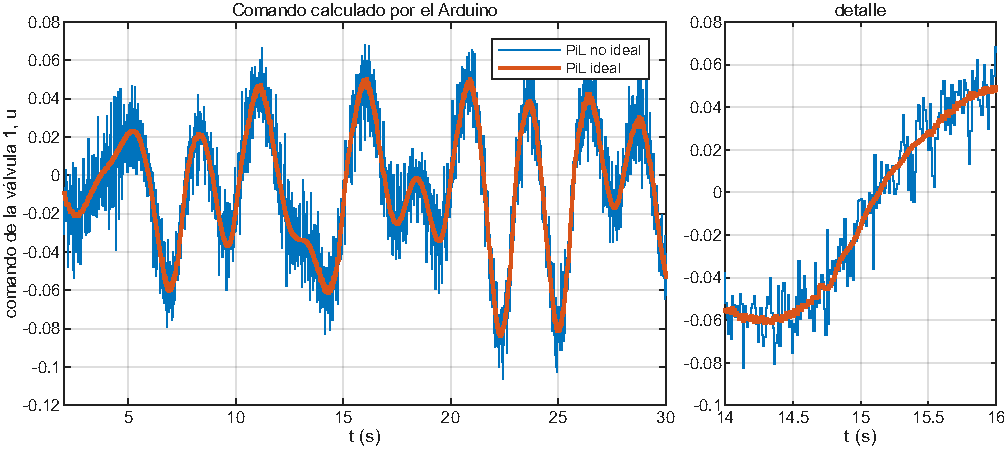
\includegraphics[width=\columnwidth]{pil_comando.pdf}
\caption{Comando de la válvula 1 calculado por el Arduino, sin y con las no idealidades del sensor ($K=15$, $H_s=\SI{2}{m}$). A la derecha, detalle de \SI{2}{s}.}
\label{fig:comando}
\end{figure}

% =====================================================================
\section{Resultados y análisis comparativo}
\label{sec:resultados}
% Criterio R3: MiL vs PiL ideal vs PiL no ideal, con métricas y conclusiones.
La Tabla~\ref{tab:resultados} y la Fig.~\ref{fig:resultados} comparan los casos durante \SI{30}{s}, sin contar los primeros \SI{2}{s} de arranque de los pistones.

\begin{table}[H]
\centering
\caption{Inclinación de la mesa ($H_s=\SI{2}{m}$, $K=15$, \SI{30}{s}). La atenuación es la del valor RMS de \textit{pitch} respecto del caso sin compensar}
\label{tab:resultados}
\footnotesize
\setlength{\tabcolsep}{3pt}
\begin{tabularx}{\columnwidth}{lCCCCC}
\toprule
Caso & Pico \textit{pitch} (\si{\degree}) & RMS \textit{pitch} (\si{\degree}) & Pico \textit{roll} (\si{\degree}) & RMS \textit{roll} (\si{\degree}) & Aten. (dB) \\
\midrule
Sin compensar ($K=0$) & 2.878 & 1.434 & 1.522 & 0.561 & --- \\
MiL & 0.784 & 0.382 & 0.418 & 0.149 & $-11.5$ \\
PiL ideal & 0.784 & 0.382 & 0.418 & 0.149 & $-11.5$ \\
PiL no ideal & 0.823 & 0.376 & 0.534 & 0.154 & $-11.6$ \\
Requisito & 1 & --- & 1 & --- & --- \\
\bottomrule
\end{tabularx}
\end{table}

\begin{figure*}[t]
\centering
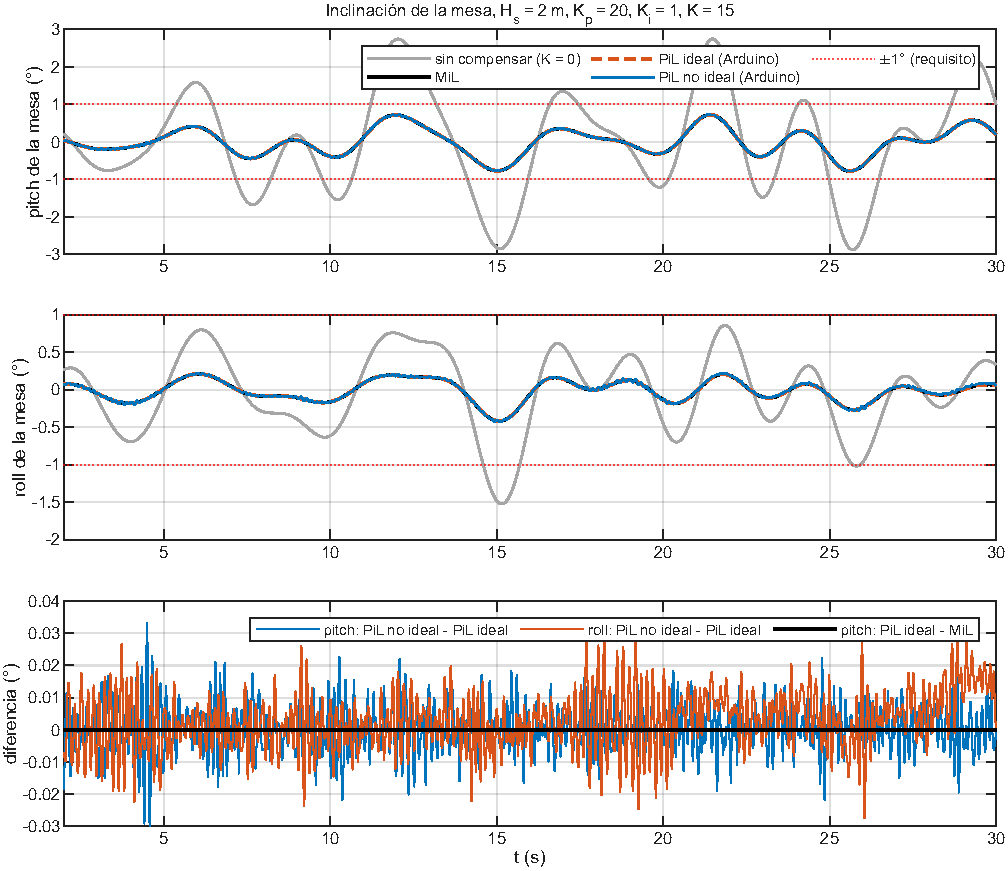
\includegraphics[width=0.85\textwidth]{pil_nivelacion.pdf}
\caption{Inclinación de la mesa en \textit{pitch} y en \textit{roll} con $H_s=\SI{2}{m}$: sin compensar, MiL, PiL ideal y PiL no ideal (los tres últimos se superponen). Abajo: efecto de las no idealidades (PiL no ideal menos PiL ideal) y diferencia entre el PiL ideal y el MiL, que es nula. Generada con \texttt{figuras/fig\_final.m}.}
\label{fig:resultados}
\end{figure*}

El lazo de nivelación reduce la inclinación de la mesa 3.7 veces (\SI{-11.5}{dB}) en pico y en valor RMS, tanto en \textit{pitch} como en \textit{roll}: el pico de \textit{pitch} pasa de \SI{2.88}{\degree} a \SI{0.78}{\degree}, por debajo del requisito de \SI{1}{\degree}, y el de \textit{roll} de \SI{1.52}{\degree} a \SI{0.42}{\degree}. La atenuación coincide con la que predice~\eqref{eq:sensibilidad}, $1/(1+15\times0.184)=0.27$. El PiL ideal y el MiL son idénticos, y las no idealidades del encoder agregan a la inclinación un ruido de \SI{0.04}{\degree} RMS (\SI{0.16}{\degree} como máximo), visible en la Fig.~\ref{fig:resultados}, sin sacar a la mesa del requisito. El esfuerzo de control es bajo: el comando RMS más alto es de \num{0.066}, y ninguna válvula satura.

\subsection{Estados de mar más agresivos}
\label{sec:oleaje}
Con $H_s=\SI{2}{m}$ y $T_p=\SI{10}{s}$ la base apenas supera \SI{3}{\degree}. Según~\eqref{eq:eta} y~\eqref{eq:pendientes}, la pendiente de la superficie crece con $k_n=\omega_n^2/g$, es decir, como $H_s/T_p^2$: subir $H_s$ la aumenta solo en proporción, mientras que acortar el periodo la aumenta con el cuadrado. Evaluando fuera de Simulink la misma función del bloque de oleaje, se fijó $H_s=\SI{2}{m}$ y se eligieron tres periodos que dan picos de \SIlist{5;10;15}{\degree} en la base: $T_p=\SIlist{7.5;5.3;4.3}{s}$. El caso de \SI{4.3}{s} es un mar muy empinado, cerca del límite de rompiente. Con el mismo controlador ($K=15$) se corrió cada caso sin compensar, en MiL y en PiL no ideal (Tabla~\ref{tab:oleaje}, Fig.~\ref{fig:oleaje}).

\begin{table}[H]
\centering
\caption{Inclinación de la mesa con oleajes más agresivos ($H_s=\SI{2}{m}$, $K=15$, \SI{30}{s}). Pico y RMS de \textit{pitch}; $u_{RMS}$ y porcentaje de tiempo saturado de la válvula más exigida}
\label{tab:oleaje}
\footnotesize
\setlength{\tabcolsep}{3pt}
\begin{tabularx}{\columnwidth}{lCCCC}
\toprule
Caso & Pico (\si{\degree}) & RMS (\si{\degree}) & $u_{RMS}$ & Sat. (\si{\percent}) \\
\midrule
\multicolumn{5}{l}{$T_p=\SI{7.5}{s}$ (\SI{5}{\degree})} \\
\quad Sin compensar & 5.11 & 2.38 & --- & 0 \\
\quad MiL & 1.46 & 0.65 & 0.074 & 0 \\
\quad PiL no ideal & 1.47 & 0.63 & 0.093 & 0 \\
\multicolumn{5}{l}{$T_p=\SI{5.3}{s}$ (\SI{10}{\degree})} \\
\quad Sin compensar & 10.14 & 4.55 & --- & 0 \\
\quad MiL & 16.63 & 4.38 & 0.45 & 11 \\
\quad PiL no ideal & 15.13 & 3.92 & 0.45 & 12 \\
\multicolumn{5}{l}{$T_p=\SI{4.3}{s}$ (\SI{15}{\degree})} \\
\quad Sin compensar & 15.15 & 6.56 & --- & 0 \\
\quad MiL & 19.97 & 7.65 & 0.53 & 18 \\
\quad PiL no ideal & 24.58 & 7.82 & 0.67 & 29 \\
\bottomrule
\end{tabularx}
\end{table}

\begin{figure*}[t]
\centering
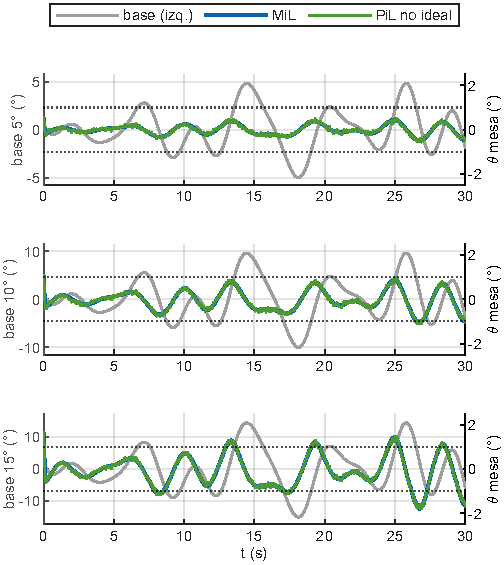
\includegraphics[width=0.85\textwidth]{oleaje_casos.pdf}
\caption{\textit{Pitch} de la mesa con los tres estados de mar de la Tabla~\ref{tab:oleaje}: sin compensar, MiL y PiL no ideal (Arduino), con $K_p=20$, $K_i=1$ y $K=15$. Generada con \texttt{figuras/fig\_oleaje.m}.}
\label{fig:oleaje}
\end{figure*}

Con \SI{5}{\degree} el lazo atenúa lo mismo que con el oleaje nominal (\SI{-11.2}{dB}, como predice~\eqref{eq:sensibilidad}), pero la mesa llega a \SI{1.46}{\degree} y no cumple el requisito: para \SI{1}{\degree} haría falta $K\ge(5.1-1)/0.184\approx22$, cerca del límite de estabilidad (con $K=30$ el lazo es inestable). Con \SIlist{10;15}{\degree} el lazo deja de nivelar: los primeros segundos sigue al caso de \SI{5}{\degree}, pero en cuanto la base supera unos \SI{6}{\degree} el comando de ángulo se satura en \SI{\pm0.6}{rad}, que con $g=0.188$ equivale a solo \SI{6.5}{\degree} de compensación, y las válvulas pasan entre el 11 y el \SI{29}{\percent} del tiempo saturadas. La mesa queda peor que sin compensar (picos de \SIrange{15}{25}{\degree}). Con este controlador, MARLUP cumple el requisito hasta unos \SI{3.7}{\degree} de perturbación ($1+0.184\cdot15$ veces \SI{1}{\degree}) y deja de estabilizar por encima de unos \SI{6}{\degree}; ampliar ese rango exige corregir la cinemática (Sec.~\ref{sec:ganancias}) y rediseñar el lazo exterior para la ganancia real.

% =====================================================================
\section{Conclusiones}
\label{sec:conclusiones}
\begin{itemize}
\item Se identificó la función de transferencia del actuador sobre el modelo no lineal, $G(s)=0.636\,e^{-0.0088s}/[s(0.0085s+1)]$, y con ella se diseñó un único PI para los tres cilindros, $K_p=20$, $K_i=1$, que cumple las especificaciones con $M_p=\SI{2.4}{\percent}$ y $t_s=\SI{0.28}{s}$ en señal pequeña, y márgenes de \SI{16.9}{dB} y \SI{73.7}{\degree}.
\item El controlador de los tres pistones, generado por Embedded Coder desde \texttt{ctrl\_pi3.slx} y ejecutado en el ATmega328P, reproduce exactamente la simulación en el PC: RMSE de \SI{0.0000}{\degree} y error máximo nulo en \SI{30}{s} de oleaje, con la plataforma completa en Simulink y un solo bloque Model en modo PIL.
\item Con oleaje de $H_s=\SI{2}{m}$ y $K=15$, el lazo de nivelación reduce el pico de inclinación de \textit{pitch} de \SI{2.88}{\degree} a \SI{0.78}{\degree} (\SI{-11.5}{dB}) y el de \textit{roll} de \SI{1.52}{\degree} a \SI{0.42}{\degree}, por debajo del requisito de \SI{1}{\degree}. Para lograrlo se amplió la saturación del comando de ángulo a $\pm\SI{0.6}{rad}$.
\item Las cuatro no idealidades del encoder lineal, en el lazo de realimentación (linealidad, histéresis, ADC de 10 bits y ruido de 5 LSB), agregan ruido de \num{0.058} RMS al comando de las válvulas y de \SI{0.04}{\degree} RMS a la inclinación de la mesa, cuyo pico de \textit{pitch} sube de \SI{0.78}{\degree} a \SI{0.82}{\degree}: el lazo interno filtra buena parte del ruido y el lazo exterior corrige los errores de posición.
\item La perturbación crece como $H_s/T_p^2$. Con $H_s=\SI{2}{m}$ y $T_p=\SIlist{7.5;5.3;4.3}{s}$ la base se inclina \SIlist{5;10;15}{\degree}. El controlador actual atenúa \SI{-11}{dB} el caso de \SI{5}{\degree} (\SI{1.46}{\degree} en la mesa, fuera del requisito) y no estabiliza los de \SIlist{10;15}{\degree}, porque solo puede compensar unos \SI{6.5}{\degree} y las válvulas se saturan.
\item El factor $g=0.188$ entre el ángulo ordenado y el realizado se explica por la geometría: el ensamble tiene un solo pasador en la unión superior de cada pata y la mesa gira alrededor del centro de la base, de modo que $g=R_T/R_B$.
\end{itemize}

Como limitaciones, el ángulo de la mesa se mide idealmente en la simulación, la ejecución en \textit{lockstep} no representa la latencia real de la UART ni la variabilidad del tiempo de cómputo, y el bloque de oleaje recorta la dispersión direccional. Como trabajo futuro se propone corregir la cinemática inversa para el mecanismo real (o el ensamble para la cinemática), rediseñar el lazo exterior para la ganancia resultante, modelar el sensor de inclinación con sus no idealidades y medir el tiempo de ejecución del controlador en el MCU frente al periodo de \SI{10}{ms}.

% =====================================================================
\begin{thebibliography}{9}
\bibitem{pil_unitario} A. Salas, M. Solís y E. Valle, ``MARLUP: Actividad 3 -- Desarrollo de sistema Processor-in-the-Loop (validación unitaria de un actuador)'', 2026.
\bibitem{avance2} A. Salas, M. Solís y E. Valle, ``MARLUP: Avance 2'', 2026.
\bibitem{rexroth} Bosch Rexroth AG, ``Hydraulic cylinder, mill type, series CDH1/CGH1,'' hoja de datos RE 17331/09.05, 2005.
\bibitem{pierson1964} W. J. Pierson y L. Moskowitz, ``A proposed spectral form for fully developed wind seas based on the similarity theory of S. A. Kitaigorodskii,'' \textit{Journal of Geophysical Research}, vol.~69, no.~24, pp.~5181--5190, 1964.
\bibitem{merritt} H. E. Merritt, \textit{Hydraulic Control Systems}. Nueva York: Wiley, 1967.
\bibitem{atmega328p} Microchip Technology Inc., ``ATmega328P 8-bit AVR Microcontroller with 32K Bytes In-System Programmable Flash,'' hoja de datos DS40002061B, 2020.
\bibitem{wang2025} W. Wang, Y. Ning, Y. Zhang, P. Xu y B. Li, ``Linear active disturbance rejection control with linear quadratic regulator for Stewart platform in active wave compensation system,'' \textit{Applied Ocean Research}, vol.~156, art.~104469, 2025. [En línea]. Disponible: \url{https://doi.org/10.1016/j.apor.2025.104469}
\end{thebibliography}

% =====================================================================
\appendix
\section*{Anexo: reproducibilidad}
Repositorio: \url{https://github.com/aasalas/LAB-DE-CONTROL-GR5}, rama \texttt{develop}. Modelo de la plataforma: \texttt{MODELOS/CINEMATICA/Model\_aaronC.slx}, con parámetros en \texttt{MARLUP\_hydr\_params.m}. PiL de los tres pistones: controlador \texttt{ctrl\_pi3.slx}, configuración \texttt{config\_pil3.m} y corridas con \texttt{correr\_pil3.m}; los pasos para reproducirlo, y una bitácora, están en el \texttt{README.md}. Escenario final (MiL y PiL, $H_s=\SI{2}{m}$, $K=15$): \texttt{MODELOS/CINEMATICA/exp2\_final.m}; datos en \texttt{DOCS/AVANCES/AVANCE 3/resultados/exp2\_final.mat} y figuras con \texttt{figuras/fig\_final.m}. Diseño del PI: \texttt{MODELOS/PISTON/diseno\_pi.m}. Plan y resultados de los experimentos: \texttt{MODELOS/CINEMATICA/BITACORA.md}. Modelo matemático del actuador: \texttt{MODELOS/PISTON/MODELO\_MATEMATICO.md}. Validación unitaria de un actuador: \texttt{MODELOS/PISTON} y \texttt{DOCS/INFORME\_PIL}.

\end{document}
